\chapter{Results}
%Plan
We begin this section with canonical results from the simulator, exploring the crux of all signal corruptions implemented. Following this, we contrast these results to real VLBA 87GHz observations of Sgr~A* and calibrators. In this analysis, we focus identifying ISM and tropospheric contributions to the data. We end with more sophisticated results of calibrator and imaging tests of a variable source within the context of a variable troposphere, with possibly some ISM thrown in.



\section{Canonical simulations}\label{sec:can_sim}
%Pr 1 St 2

%

%ISM_sequence 
To demonstrate the implementation and provide an example of intraday ISM variability, we present the results of a simulated observation of 10 minutes duration at 14:00 UTC on four consecutive days in Fig.~\ref{ISM_sequence}. To compare to published observations, we use the three-station EHT array consisting of the Submillimeter Telescope (SMT) in Arizona, the Combined Array for Research in Millimeter-wave Astronomy (CARMA) in California and the James Clerk Maxwell Telescope (JCMT) on Mauna Kea, Hawaii. The distance to the screen is taken as $D_{\rm os}=5.8 \pm 0.3$~kpc  \citep{Bower_2014}. The relative transverse velocity between the observer and scattering screen is set to $50~\rm{km\,s}^{-1}$ to be consistent with \citet{2016arXiv160106571O}. The source is a circular Gaussian with a $\rm{FHWM}=40$~$\mu$-arcsec, approximately the angular distance that a scattering screen would travel over $\sim 4$~days. The source size has been chosen such that it is consistent with the latest estimate of the size of Sgr~A$^\star$ at $230$~GHz \citep{Fish_2011}.  Closure quantities are model dependent and calculated as specified in \citet{Rogers_1995}, where the thermal noise was added based on the system equivalent flux density (SEFD) table in \citep{Lu_2014}. 

\begin{figure*}
\begin{center}
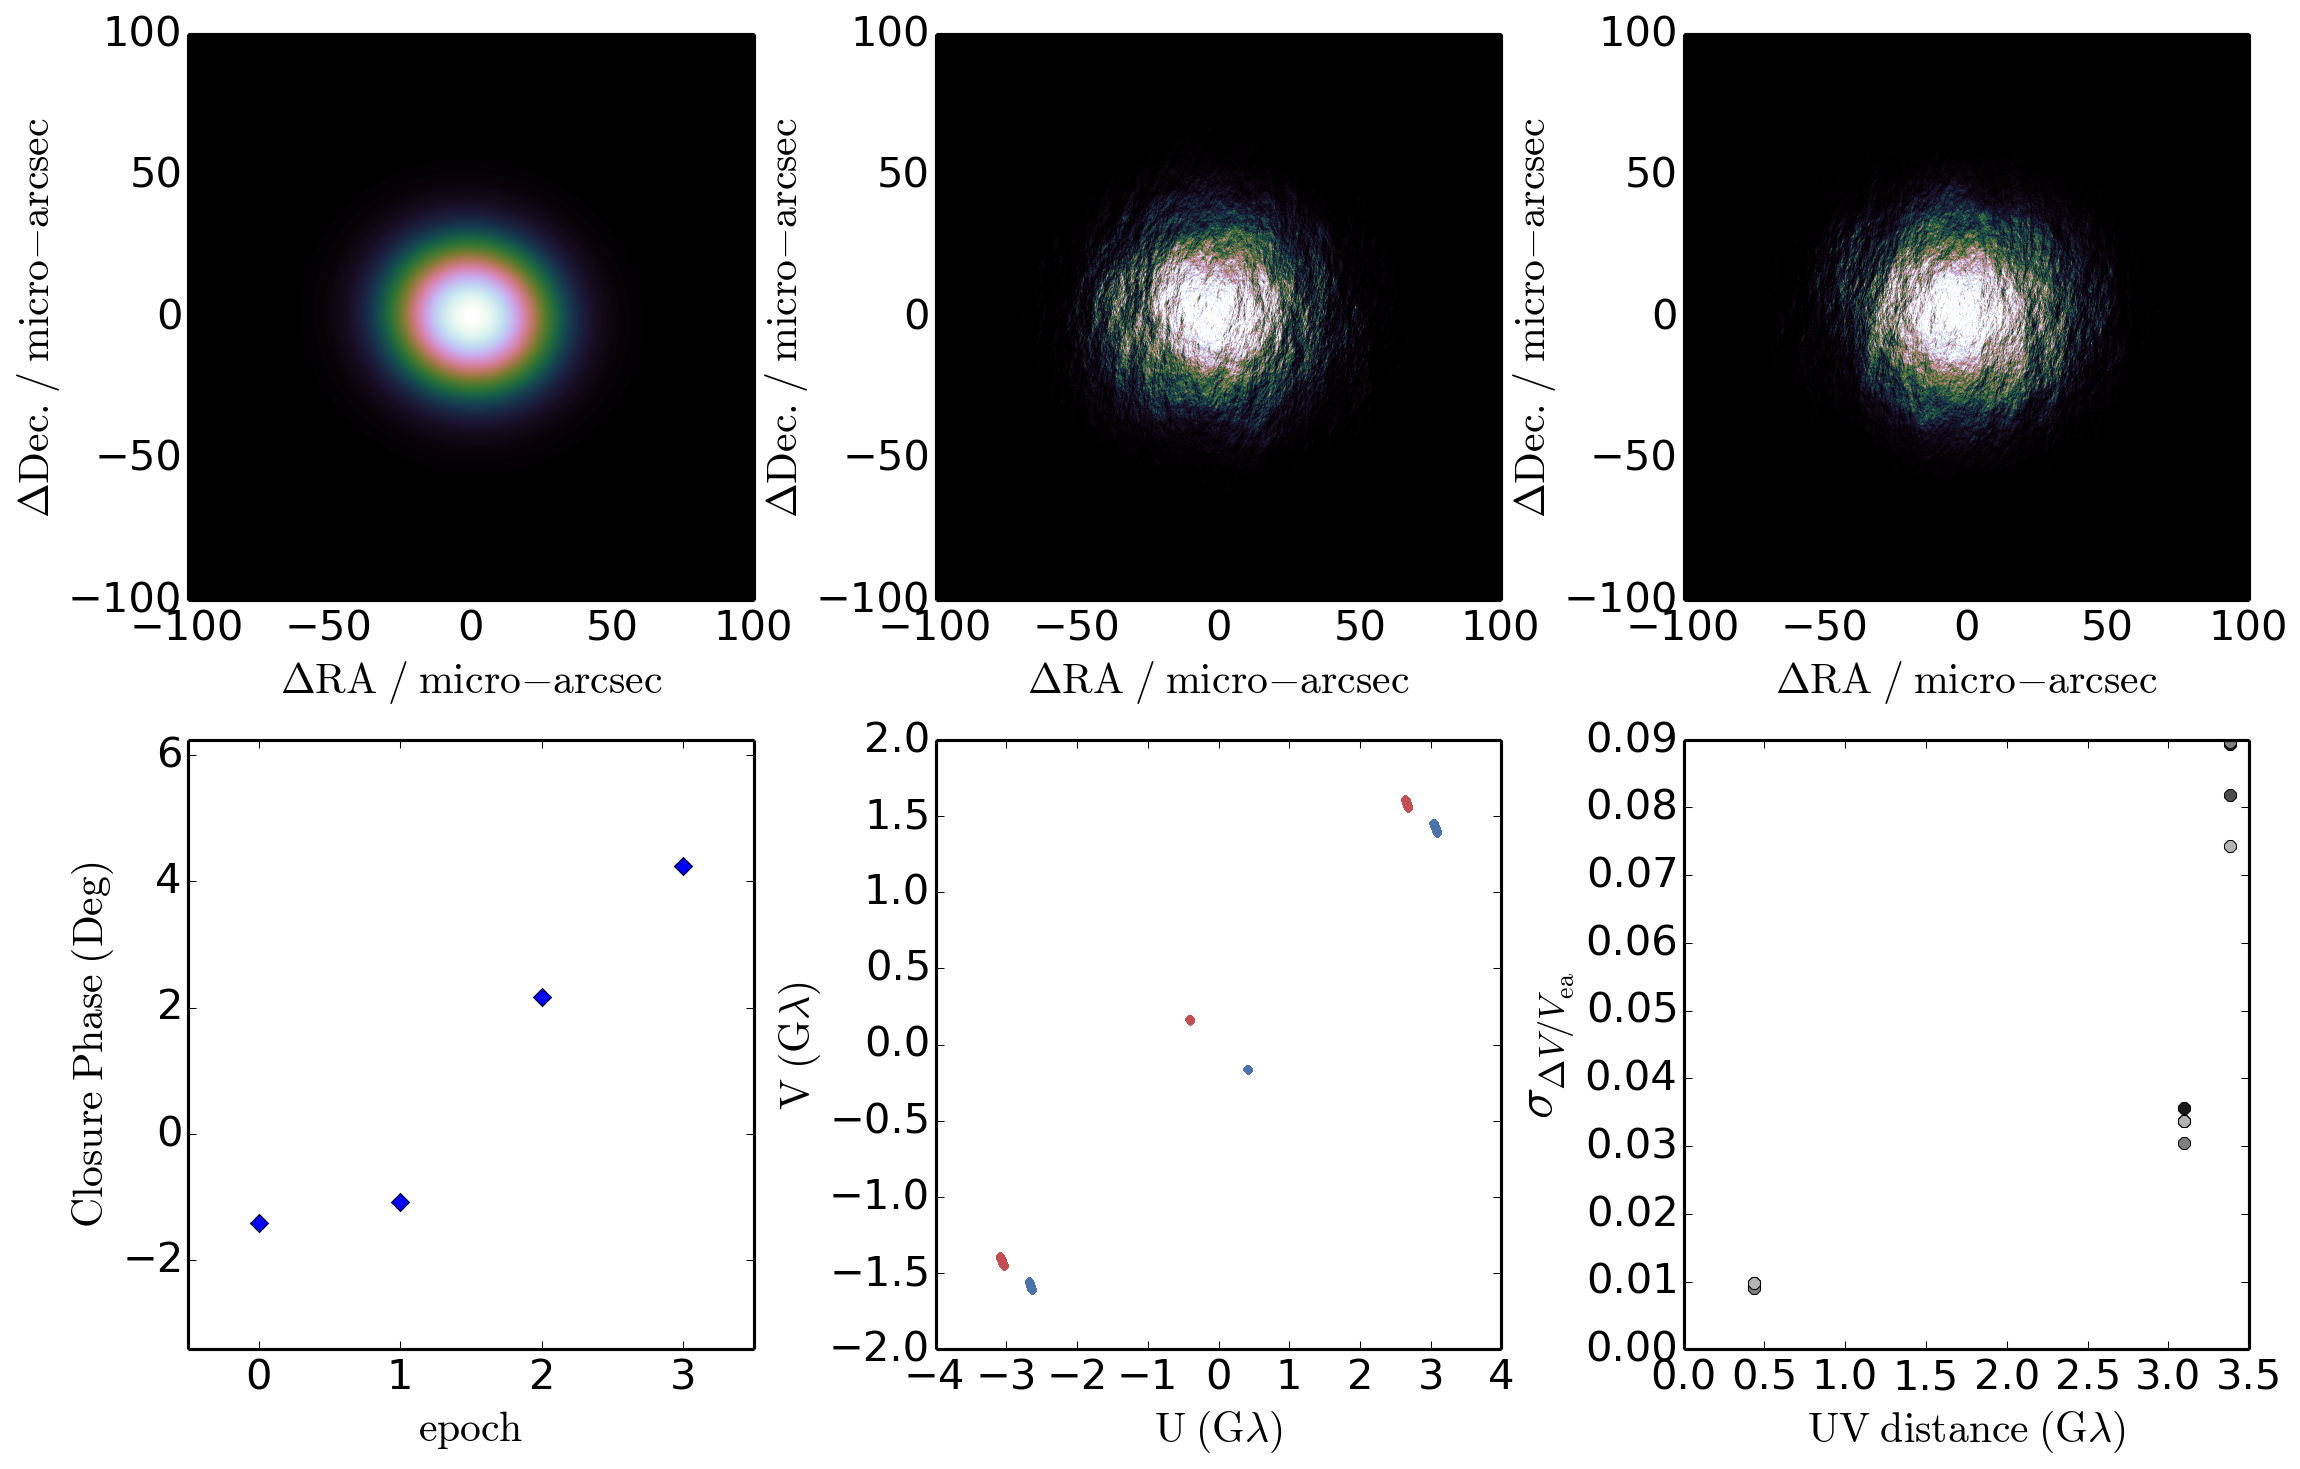
\includegraphics[width=1.8\columnwidth]{Images/ism}
\caption{An example simulation of ISM scattering towards Sgr~A$^{\star}$, observed with SMT-JCMT-CARMA.  The top panel, left to right, shows the original $\rm FWHM = 40$~$\mu$-arcsec Gaussian {\bf (top left)}, the simulated ISM scattered image on the first night {\bf (top middle)} and last night {\bf (top right)} of the observation, respectively.  The bottom panel, left to right,  shows the evolution of the 10 minute-averaged closure phase with epoch {\bf (bottom left)}, {\sl uv}-tracks for each night {\bf (bottom middle)} and the RMS fractional visibility amplitude differences $\sigma_{\Delta V /V_{\rm ea}}$ as a function of {\sl uv-}distance {\bf (bottom right)}. $ \Delta V= (|V_{\rm a}|-|V_{\rm ea}|)$, where $|V_{\rm a}|$ and |$|V_{\rm ea}|$ are the simulated average and ensemble average visibility amplitudes respectively. Variations from the ensemble-average flux on the shortest baselines reveal total flux modulation while flux variations on longer baselines and non-zero closure phases track the fluctuations in substructure.  Furthermore, ISM scattering simulations can constrain the variability fraction associated with the screen, enabling a more robust estimation of source variability, as demonstrated in \citet{2016arXiv160106571O}. The time-variability of the ISM is built into the {\sc MeqSilhouette} framework.\label{ISM_sequence}%
}
\end{center}
\end{figure*}

%Opacity + Brightness temperature
Typical opacities and sky brightness temperatures for ALMA, the Submillimeter Array (SMA) and the South Pole Telescope (SPT)  are shown in Fig.~\ref{fig:mean_atm}.  Note that both the opacity and brightness temperature are inversely proportional to the ground temperature and proportional to ground pressure.

\begin{figure}
\begin{center}
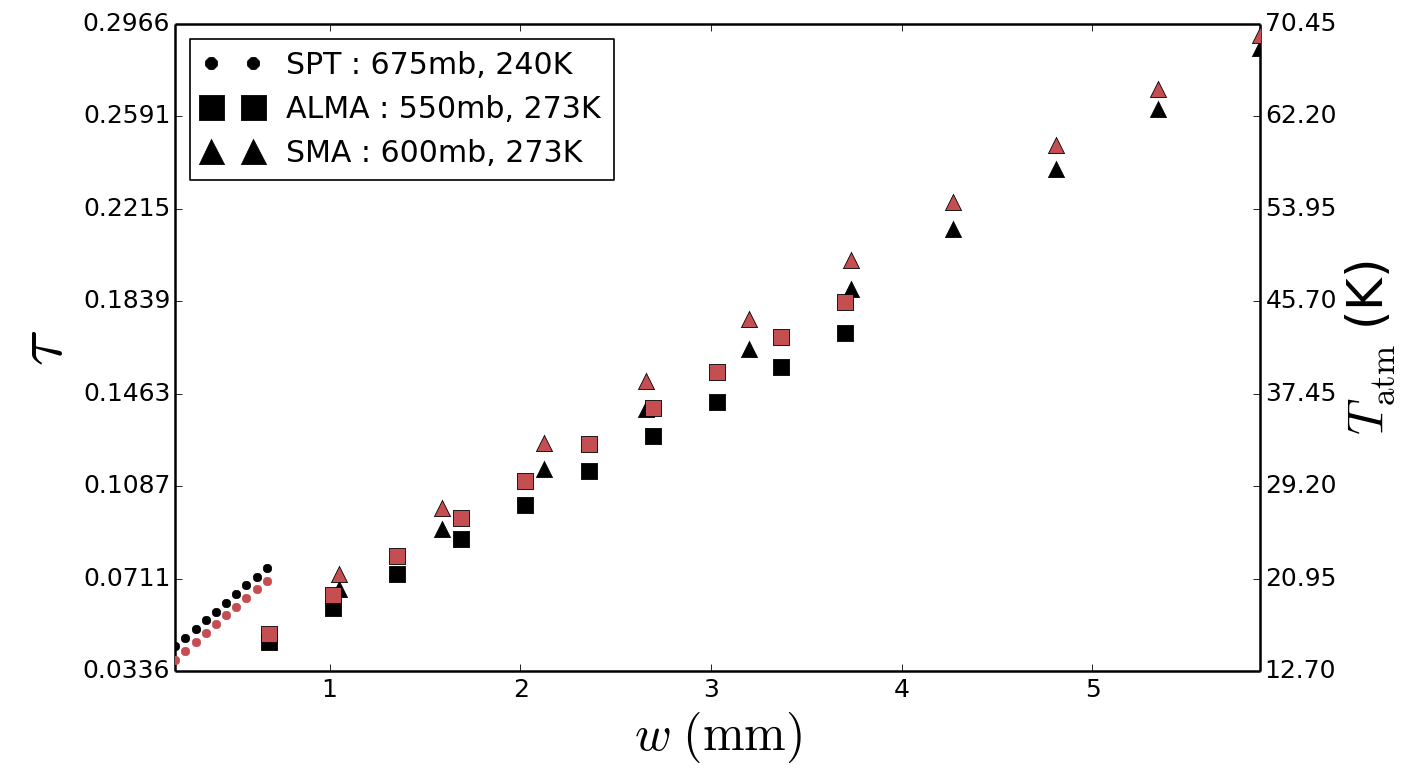
\includegraphics[width=1.\columnwidth]{Images/opacity}
\caption{Simulated mean opacity (black) and sky brightness temperature (red) at $\nu =230$~GHz  for three typical ground pressures and temperatures over a typical PWV range \citep{Lane_1998} which approximately represent the sites of SPT (dots), ALMA (squares) and SMA (triangles). The legend shows the estimated input ground (pressure, temperature) parameters for each site.\label{fig:mean_atm}%
}
\end{center}
\end{figure}


\begin{figure}
\begin{center}
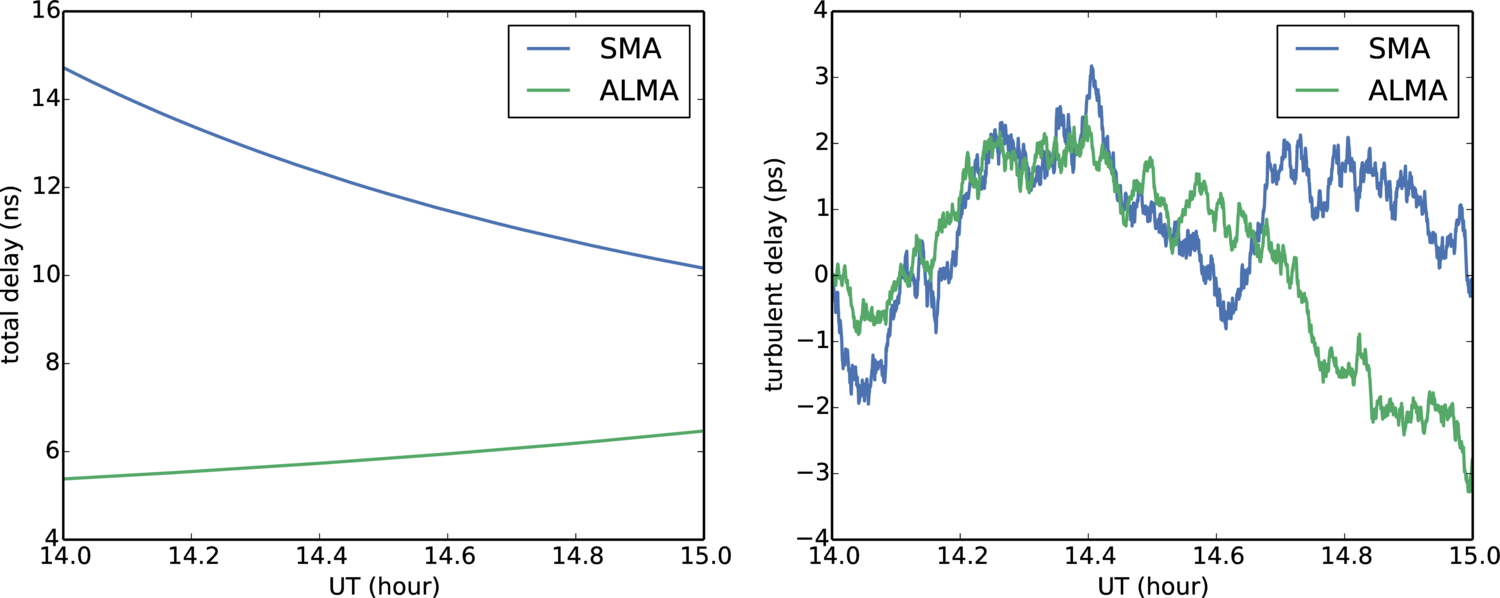
\includegraphics[width=\columnwidth]{Images/delays}
\caption{Simulation of the total delay (left) and the turbulent atmospheric delay (right) for SMA (blue) and ALMA (green) sites towards Sgr~A$^\star$. Ground pressures and temperatures are the same as Fig.~\ref{fig:mean_atm}, precipitable water vapour above each station is set to $w=2$~mm, and the instantaneous zenith coherence time is set $T_0=10$~s for both stations. Note that all tropospheric parameters are, however, independently set. The conversion from time delay to phase at 230~GHz is $1$~rad~$=0.7$~ps.\label{delay_plots}%
}
\end{center}
\end{figure}


\begin{figure*}
\begin{center}
\includegraphics[width=\columnwidth]{Images/trop_images}
\caption{The effect of residual troposphere phase noise on interferometric images of a point source observed for 12 hours at 230~GHz with 4~GHz bandwidth with the following array : SPT, ALMA, SMA, SMT, LMT and JCMT, assuming the same SEFDs as \protect\citet{Lu_2014} and an elevation limit of 15$^\circ$. For simplicity the weather parameters at each station were set to: coherence time $t_{\rm 0}=10$~sec; PWV depth $w=1$~mm; ground pressure $P=600$~mb; ground temperature $T =273$~K. {\bf Top left:} interferometric map with thermal noise only. {\bf Top right:} atmospheric attenuation and sky noise (due to non-zero opacity) with 1\% of the turbulent phase noise added. {\bf Bottom left:} as previous but with 3\% of turbulent phase contribution. {\bf Bottom right:} as previous but with 6\% turbulent phase contribution. The fractional turbulent phase contributions are illustrative of the effect of fringe-fitting errors. Note the decrease in the source peak flux with increasing turbulent tropospheric phase noise. Note further that the peak source centroid is offset from its true position (black crosshairs). \label{fig:trop_images}%
}
\end{center}
\end{figure*}


\begin{figure}
\begin{center}
\includegraphics[width=\columnwidth]{Images/point_Crop}
\caption{RMS relative amplitude error induced by pointing error with the 50~m (i.e. fully illuminated) LMT antenna as a function of pointing error offset $\rho$ at 230~GHz. We assume that these errors are degenerate or non-separable from the self-calibration/fringe-fitting model used. See text for the description of the three models used. This simulation capability enables constraints on the magnitude of pointing-induced errors given a particular pointing calibration strategy.\label{fig:pointing}%
}
\end{center}
\end{figure}


{\bf Tropospheric induced closure phase errors}
!!A bug which came from averaging
 
 
In this paper, we present the first release of the \textsc{MeqSilhouette} synthetic data simulation package. The pipeline is optimised towards mm-VLBI, taking into account user-specified stages of the signal propagation path, which enables the quantification of a range of systematic effects. Focus has been placed on modeling the effects of signal transmission through the ISM and troposphere as well as instrumental errors (i.e. pointing error and thermal noise). Time variability in all relevant domains (source, array, ISM, troposphere) is implemented. The run time for a typical simulation with a realistic instrumental setup is on the order of minutes.  Implementation of polarisation effects is intended in the next release. 


The ISM scattering implementation \textsc{ScatterBrane}, based on \citet*{Johnson_2015a}, has been incorporated into the pipeline. Fig.~\ref{ISM_sequence} provides an example of closure phase and flux variability over a 4 day period using a static source. Accurate simulation of the ISM-induced closure phase variation is essential in order to make any inference on asymmetric, event-horizon scale structure \citep[e.g.][]{Fish_2016,2016arXiv160106571O}. This will become even more important as the EHT sensitivity increases by an order of magnitude in the near future. Note that if the source has intrinsic spatial variability as in the case of a hotspot model \cite{Doeleman_2009}, this will increase ISM variability as the relative motion between source, screen and observer is increased. 


In section~\ref{sec:pointing}, we show how antenna pointing errors of the LMT could introduce fractional RMS amplitude variations $\sigma_{\Delta V/V_0} \le 0.4$ on the timescale of phase centre switching. This would occur if the calibrator is widely separated from the source, as is often the case in mm-VLBI. In contrast tracking errors are less problematic with $\sigma_{\Delta V/V_0} \le 0.05$. If the gain error is non-separable from the calibration model used, it could be interpreted as intrinsic variability, substructure and/or increased noise. If unaccounted for, this effect has the potential to limit the dynamic range of mm-VLBI images. Further tests to constrain the pointing uncertainties of EHT stations will lead to more accurate interferometric simulations and hence the overall impact on black hole shadow parameter estimation. Here we demonstrate the capability to incorporate a range of plausible pointing error effects into a full simulation pipeline.  


In section~\ref{sec:trop_errors} we explore the observational consequences of observing through a turbulent troposphere. In this simulation, we assume a simple point source model and apply increasing levels of turbulence-induced phase fluctuations before imaging using the two dimensional inverse fast Fourier transforms. We note a rapid attenuation in peak flux due to incoherent averaging, slight offsets in the source centroid and the presence of spurious imaging artefacts. Suprisingly, in this configuration, there was no evidence of blurring or a loss of resolution with the uncertainties. In an upcoming paper, we perform a systematic exploration of the turbulent tropospheric effects on the accuracy of fringe-fitting algorithms/strategies, through use of an automated calibration procedure and including the added complexity of a time-variable source. 

Significant progress has been made in the theoretical and numerical modeling of the inner accretion flow and jet launch regions near a supermassive black hole event horizon. With \textsc{MeqSilhouette}, we now have the ability to couple these with sophisticated interferometric and signal propagation simulations. This offers a tool to enable a more closely-knit and effective interplay between theoretical predictions and observational capabilities. Moreover, detailed interferometric simulations will enable us to quantify systematic effects on the black hole and/or accretion flow parameter estimation.
 

\section{A comparison to real data}

%intention
We now seek to explore a real dataset to make a first order comparison with the assumptions and predictions of our model. Currently EHT datasets are not public, so we have opted to use a 3.5~mm VLBA dataset from the public, online VLBA archive. We chose an observation of SgrA* and nearby calibrator NRAO530. 

%plan 
We begin with an exploration the decoherence properties of the visibility phase which we compare with our atmospheric turbulence module. 


\subsection{Phases and coherence}

%Coherence times 
In our canonical simulations (section~\ref{can:sim}) we assumed a constant zenith coherence time of $t_0 = 10$~s throughout the duration of the observation.  Scaling up to 3.5~mm, this translates to $t_0 \approx 25$~s, with the caveat that, on average, EHT stations are situated in locations with more stable atmospheres than VLBA stations . Fig.~\ref{fig:coherence} shows a normalised histogram of coherence times towards NRAO530 for all baselines and scans. We find a mean and standard deviation of the coherence times to be $(\mu, \sigma)_{\rm t_0} = (8.87,6.09)$.

\begin{figure}
\begin{center}
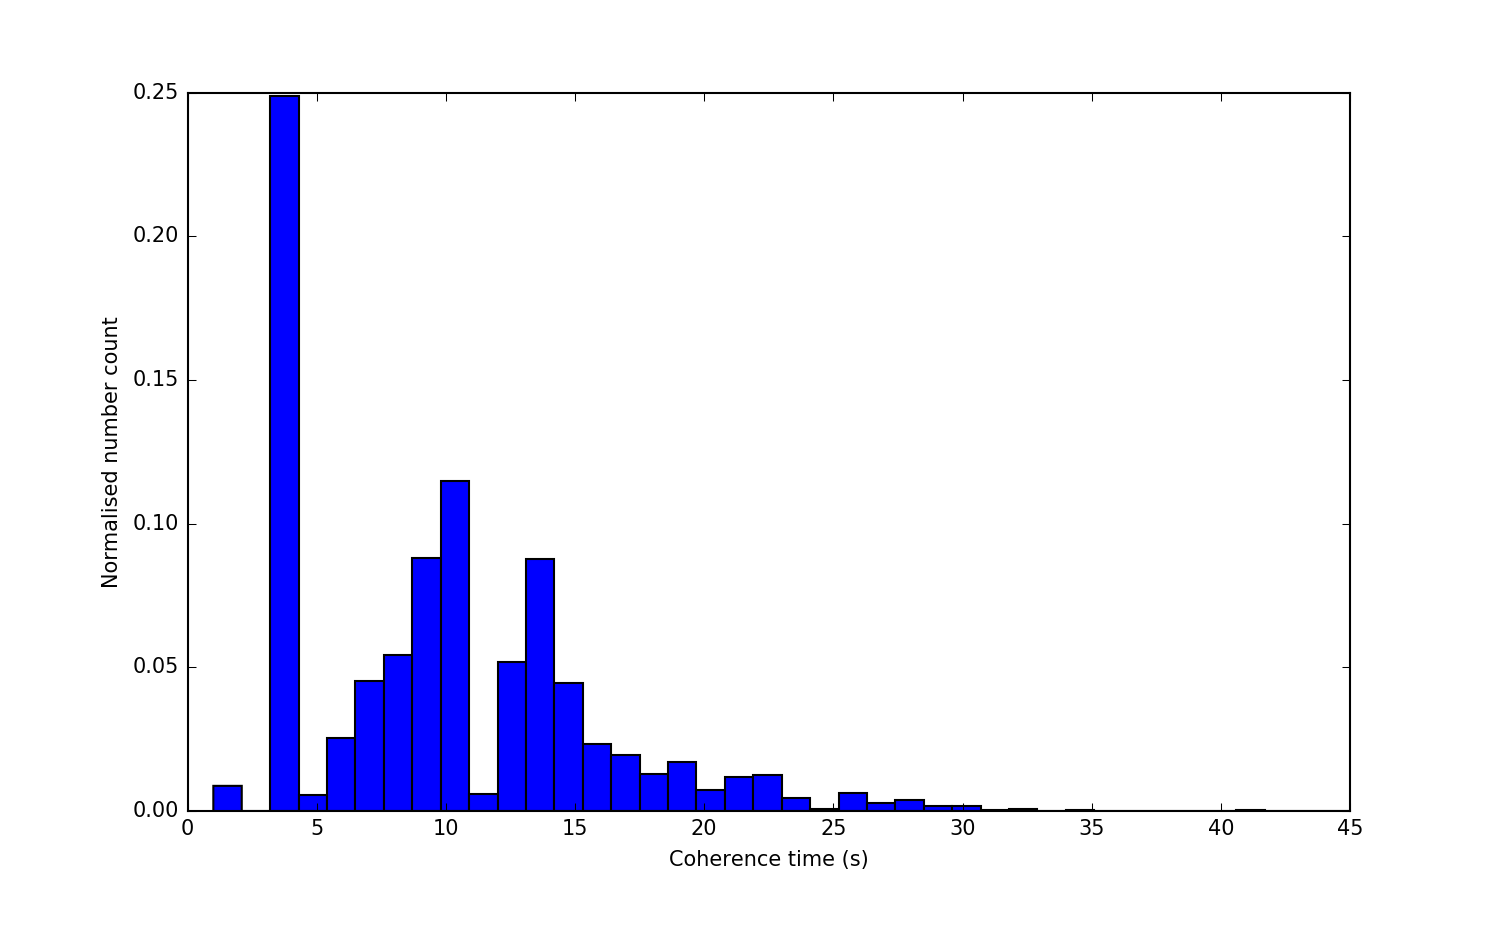
\includegraphics[width=\columnwidth]{Images/Coherence_time_NRAO530ff}
\caption{Normalised histogram of the coherence times for 87~GHz VLBA observation of NRAO530. The coherence times were generated using the {\sc aips} {\sc coher} task. The mean and standard deviation of the coherence times, $(\mu, \sigma) = (8.87,6.09)$. \label{fig:coherence}%
}
\end{center}
\end{figure}


An inspection of the observation weather tables shows a ground windspeed  $(\mu, \sigma)_v = (2.5, 1.8)$~m/s. This speed is too low to account for the above coherence time and hence indicates that most of the turbulence originates higher up in the troposphere.

%Inspectation of the histograms of phase differences
With an estimate of the coherence and assuming the canonical value for the turbulent exponent $\beta = 5/6$, we estimate, for $t_int \approx 1$, ${\sigma_\phi \approx (t_{\int}/t_0)^{5/6} \approx 9}^\circ$. From the data, averaging over channel but taking the difference in time. This doesn't make sense without a delay search a without this it's fairly obvious that the $\sigma_\phi$ will be much higher... can one apply the delay found by AIPS COHER to the UVFITS file? 

\subsection{Closure phase} 

How large is the uncertainty on the closure phase. Is this consistent with just a thermal noise prediction?


\subsection{Amplitude}

What is the variability in the visibility amplitude? How significant is the stochastic variation? How does it compare to thermal noise?

Are there any obvious systematics in the data? how much would I expect antenna pointing or troposphere to contribute


\section{Calibration and imaging of a time variable source in the presence of the troposphere}

First we fringe fit and image a stationary point source and compare to the result in Fig.~\ref{fig:trop_images}. 








